\title{Theory}

\documentclass[11pt]{article}
\usepackage[utf8]{inputenc}
\author{
        Kasper Videbæk \\
}
\date{\today}
 \usepackage{amsmath}
\usepackage{graphicx}
\usepackage[numbers]{natbib}
\usepackage{todonotes}
\usepackage[hidelinks]{hyperref}
\usepackage{epstopdf}
\usepackage{wrapfig}
\usepackage{listings}
\begin{document}
\maketitle

\tableofcontents

\clearpage 
\section{Introduction}

\clearpage 
\section{Theory}
Several topics, scientific as well as practical, are related to the work that will be done in this thesis.

In this section I will give a brief overview of what areas we will be going through, and what related work has already been done in those areas. In the first subsection we will look into research that already have worked on embedding syntax tree knowledge into version control systems, and in the second section, we will look into tree differencing. In the last section we will look into general knowledge about merging trees.

\subsection{Version control systems}
The overall goal of version control systems is to support development of documents, by keeping track of changes over time. In the context of software development, version control systems are frequently used to keep track of source code. Two overall groups of version control systems exists: Distributed and centralized. In the context of this thesis, we do not distinguish between these two - but abstract all the different merging-scenarios possible into the simple concept of merging two branches with a common ancestor.\todo[inline]{Skrive mere om process?}

Merging in version controls is the process of producing a single file, given two files that have evolved in different directions from a common ancestor. Merging source code is an inherent part of software development, and has gone through some development and automation since the first version control systems. Merging algorithms generally work by matching content between the two branches and the common ancestor. Given these matchings it is possible to merge the content into one common child. If this is not possible, we have a conflict and it will be presented to the user.

Merging tools of version control systems are mostly line based and oblivious to the structure of the content of the files contained. They work by matching each line in the two branches with the common ancestor. Given these matchings, it will conclude which lines has been deleted and added in the two different branches, and produce single file that has all these deletions ans insertions included. If changes happen near each other, it will produce a conflict.

%Version control systems can contain any type of file. Binary files are generally not merged by version control systems. Instead they are treated as conflicts instantly. 

A line based approach to works relatively well with source files and XML files, since line breaks are often used to make the structure of the code more easily readable for users. It is common for XML files to have opening and closing XML-tags on their own lines, and conventions of most programming languages have only one statement per line and opening block on lines of their own. In some programming languages line breaks are actually a part of the structure of the code - which makes them even more suitable for this approach.

However conventions of XML or source code can be broken. An entire XML-file can be a single line, and have the exact same meaning. Likewise with most source code - a function body can be written on a single line in many programming languages, and the compiler will never notice.

\todo[inline]{Er formålet med dette speciale at fixe "ikke bruger-læsbar-merging"?}

A structured merging approach will clearly be helpful for files that are not structured with line breaks. However this is not a very common case. The better case for improving version control by introducing structural knowledge, is where a single line contains structure. \todo[inline]{Dette hører nok til et andet sted}

A conflict can be defined in quite a few ways for line based tools. In the Unix tool diff3, a conflict is a sequence of lines, that is changed in both branches, and is not separated by a single line that is unchanged in both branches. Such a conflict detection scheme is clearly an approximation. It is oblivious to the structure of the data and one could craft input that will output invalid structural data. Further, the  actual meaning of the merged data is not considered at all - even if it is structurally valid, it might semantically be nonsense, even though a conflicts is not produced.


\subsection{Automatic merging}
This can probably attributed to such an approach working relatively well with source code, XML and other files often found in repositories.

Structure matching will most definitely also be a more time consuming task, and given the general use case of some commits, it might not be worth the extra computation time. Further programs are generally undecidable which means it would be impossible to actually decide if a merge will work as intended by the user, without the user assessing it manually.

One very commonly used algorithm for merging is Diff3. \citet{Khanna} investigated it formally by regarding a file as a sequence where each line was an item in the sequence. They set up a number of expectations of what you would expect from a merge, and showed that many of these assumptions does not hold: Conflicts can happen even when only unrelated regions are changed, differencing after a merge does not produce empty output, merging fails when both branches are very different from the ancestor and so forth. Even though this is the case, Diff3 continues to be widely used with few complaints of it shortcomings - it seems that the situations where Diff3 breaks are quite uncommon in version control systems.

Common algorithms for merging are state based. They compare the final state of branches, and creating a series of operations that will transform one document from one state into another. \citet{Lippe} described a different approach, where editing tools instead would remember the operations used to transform the data, and where the merge process will be a matter of applying these transformations in the right order to minimize the amount of conflicts.
\todo[inline]{Mention whitespace ignoring}
\todo[inline]{Mention horizontal differincing}
\todo[inline]{Talk about prettyprinters.}
\todo[inline]{Point out that merges might not compile.}


\subsection{Programming languages}
Programming languages are abstractions over the calculations computers can perform. They makes it easier for a programmer to express the problems they need to solve, without requiring the programmer to handle intricate details about memory and processors, and they allow the user to write programs as text files, and let the computer handle the process of executing the ideas expressed in the code.

In this section we will look into the process that a program goes through, from source code to execution, to give an overview of which techniques will be used later in the thesis.

\subsubsection{Grammars}
The process of turning programs into execution relies on lexers and parsers, generated through token specifications and a context-free grammars.

A token is any concrete string of text that is legal at any point in the program text. Figure \ref{token} shows a token specification, for a very simply language, that understands numbers, strings, a couple of keywords and structural tokens like parenthesis. Strings and integers are parsed through regular expressions and 

The context free grammar is the structure that defines which tokens are valid in which sequence in the program text. At any given point of the parsing - it defines whether or not a given token is valid. Given a grammar of a language, we will be able to to parse the syntax of a legal program, or to generate syntax errors for invalid ones. Figure \ref{grammar} defines a grammar relying on the token specification in figure \ref{token}.

In combination they create a very small imperative programming language, that is mostly nonsensical outside of as an example of this section.

\begin{figure}
  \caption{An example of a simple token specification.}
  \label{token}
\begin{verbatim}
TOKEN:
    IDENTIFIER
    KEYWORD
    BOOLEAN
    NUMBER
    IDENTIFIER
    STRUCTURE
    
KEYWORD:
    IF =          "if"
    WHILE =       "while"
    FOR =         "for"
    ELSE =        "else"
    INT =         "int"
    
BOOLEAN:
    TRUE          "true"
    FALSE         "false"

NUMBER:
    {int}         "['0'-'9']+"
    
IDENTIFIER:
    {string}     "[a-zA-Z0-9]+"
    
STRUCTURE:
    LPAR =        "("
    RPAR =        ")"
    LBRACKET =    "{"
    RBRACKET =    "}"
    SEMI =        ";"
    EQUAL =       "="
    LT =          "<"
    INC =         "++"

\end{verbatim}
\end{figure}

\begin{figure}
  \caption{An example of a simple grammar.}
  \label{grammar}
\begin{verbatim}
start:
    statement list

statement:
    expression SEMICOLON
    ifstatement
    whilestatement
    forstatement
    statementblock

forstatement:
    FOR LPAR expression SEMI expression SEMI expression SEMI expression LPAR statement
    
expression:
    BOOLEAN
    identifier INC
    identifier LT NUM
    INT identifier EQUALS NUM
    
ifstatement:
    IF LPAR expression RPAR statement
    IF LPAR expression RPAR statement ELSE statement

whilestatement:
    while LPAR expression RPAR statement
    
statementblock:
    LBRACKET statement list RBRACKET
\end{verbatim}
\end{figure}

\subsubsection{Syntax Trees}
The purpose of parsing source code is often iterating over the elements of it to generate a syntax tree. A syntax tree is a tree representation of the program. The syntax tree representation is useful for further processing of the semantics of a program. At this point a lot of details about the concrete textual representation of the code has also left behind. An example of a syntax tree can be found in Figure \ref{syntaxtree}. 

Depending on what kind of choice of syntax tree is done, information of the concrete syntax might be lost. In C, for example, the construct \texttt{a[i]]} is a shorthand for \texttt{*(a + i)} and should produce the same semantic behaviour. Rewriting them both into the same structure in the syntax tree is one way to resolve this. However doing this, also means that given a syntax tree it will be harder, or impossible, to determine what the concrete syntax was.

Even grander structure rewrites could be done in the transformation from a code file to a syntax tree. For example it is possible to fit the grammar from Figure \ref{grammar} into the syntax tree of \ref{syntaxtree} even though no for-loop exists in the tree. This would be done by rewriting it into a while loop construction. Such a rewrite would of course make it quite hard to deconstruct a syntax tree back into the actual concrete code that was used to generate it.

Given the purpose of this thesis, the choice of syntax tree is quite important for us: We will constantly be looking at syntax nodes, and want to generate concrete syntax - which means we will always want a syntax tree that is as closely corresponding to the grammatical constructs of the language.

\begin{figure}
  \caption{An example of a simple syntax tree written as a F\# type.}
  \label{syntaxtree}
\begin{verbatim}


type statement =
  | EXPR of expression
  | IF of expression * statement * statement
  | WHILE of expression * statement
  | BLOCK of statement list

and expression =
  | BOOL of bool
  | INC of string
  | DEC of string * int
  | LT of string * int

and program = 
  | BODY of statement list


\end{verbatim}
\end{figure}



\subsubsection{Pre-processing and comments}
\todo[inline]{Syntax Trees and Preprocessing??}
%http://bartho.net/publications/Adding_preprocessor_directives.pdf
When looking at the syntax tree quite a lot of information will not be immediately available: Everything from the preprocessing phase, syntactic sugar, whitespace and comments. While this information is not immediately available in the structure of the syntax tree most of this information can be found, by looking at the text that generated each node in the tree. 

\subsection{Syntax Trees in Version Control}
There has been several attempts at creating more structure awareness in version control systems with several different goals. \citet{Freese} describes the idea of version control systems that would understand the code in a repository, and also have capabilities of migrating newly committed code automatically when a public API has changed.

Syntax tree differencing has generally been used to get overview of changes in version controls. \citet{Fluri} describes an approximating algorithm for trees, that  detects moves and and uses a heuristics approach to define how good a match a node is to another node - looking at both the value but also the child nodes. They also describe string similarity measures in which reordering of words in variable names will be more similar and describe use cases for this. \citet{Hashimoto} also describes the idea of analysing code through syntax trees and discuss several applications. They presents an approach that works for four different object-oriented languages, and note that too fine-grained tree-edit-scripts will actually be less comprehensible than more coarse-grained.

\citet{Hunt} describes the idea of using renaming and move-detection to avoid conflicts in language aware merging tools, and the idea of redefining the definition of conflicts to include some semantic conflicts, where the user should be warned about branches interfering in each others code. They do not provide much low level information about the algorithm.

\citet{Ekman} also looks into refactorings using the ideas of \citet{Lippe}. The idea is to log refactorings and normal code changes, they apply traditional changes first and thereafter apply refactorings. Further they discuss how preconditions can be detected and used to detect merge conflicts.

\citet{Apel} describes the idea of semistructured merge and creates a framework that will be extensible to several languages. They parse programs into unordered trees in which the leaves are functions that contain unstructured program code. The code in leaves is then merged by language specific conflict handlers or by an unstructured merge. They found that merge conflicts are generally minimized, and conclude that many conflicts are ordering conflicts. In 26\% of the cases there will actually be more conflicts, due to renaming creating conflicts in this approach as opposed to compile errors in unstructured merge.

\citet{Olav} describes a system which first tries unstructured merge and afterwords does structured merge on conflicting JAVA files. The idea is to minimize the running time of the tools, to make them more convenient to use in real life scenarios. They report generally a lower amount of conflicts than unstructured merge and \citet{Apel} but in some scenarios, in the case of moved files, they produce more conflicts. They general cut off 50\% of the running time compared to a pure structured approach, are a factor 12 slower than a unstructured merge, and a factor 6 faster than \citet{Apel}. However the improvement factor varies a lot from repository to repository. 


\subsection{Tree differencing  and merging}
Research in the area has shown that the problem generally can be solved in cubic time. Several different algorithms exists, that all build on different dynamic programming decompositions. They perform well in different circumstances, and algorithms for cubic time have been created. \citet{Pawlik} describes and algorithm that will perform in cubic time, and that dynamically will decide if other algorithms would perform better for a specific sub-problem - this algorithm seems to be the most promising in regards to differencing and running time.

\citet{Zhang} describes the idea of constraining mapping, such that the one of the common ancestors of two nodes needs to be the same. This provides and algorithm that runs in quadratic time. Later \citet{Lu} described a loosened constraint and provided an algorithm that was quadratic, but also dependant on the degree of the tree.

Merging is not a time consuming problem, as long as an edit script is provided. The different existing merging algorithms that exists for three-way merging on trees generally describe different properties that is desirable for how to resolve conflicts, or when to produce them. \citet{lindholm} describes a merging algorithm for XML documents, \citet{Horwitz,Asklund,Olav} describes merging properties interesting for program code.

\todo{Ting der arbejder på tvaers af sprog:
Semistroctored Merge: Rethinking Merge in Revision Control Systems
Diff/TS: A tool for fine grained....
}
\clearpage

\section{Discussions}
Every developer has their own preferences of development environment, which makes it essential that a tool can work with many environments, and as such a operation based approach where changes are logged by an editor, seems quite impractical, so we will keep the integration in the version control systems. 

Several people already have looked into structural differencing and merging of structured data and specifically program code. This research seems however to focus mostly on the conflict resolution part, and glances over the problem of running times. 

In this thesis, I will focus on two parts: Overcoming the running time challenge, and further creating an interface into general algorithms, that will make it easier to implement support for new languages.

\todo{Semantisk, eller ikke-semantisk tree merging? Every node behaves differently}


\subsection{Merging syntax}
In a perfect universe, the perfect merge-result would be a merge that produces either no unintended behaviour or a conflict, if the input code has no unintended behaviour. It however not possible to guarantee that a single code file has no unintended behaviour, and as such this goal is not attainable, and certainly not only looking at the syntax tree without much more in-depth semantic analysis. Further, the current tools cannot guarantee this output at all.



%http://users.soe.ucsc.edu/~ejw/scm12/papers/Hayase-Chapter10.pdf

Many different strictness levels exists across the landscape of programming languages, but even the strictest programming language will allow incorrect programs through - simply because 


\subsection{Cross-language interfaces}
Structured differencing tools will be only for specific languages or structures. This makes such tools impractical in version control systems, since they are designed to integrate with line based tools, and do not discriminate between file types. Some research has been done into making tools that will work with either several languages, or that combines a line based approach with a structured approach.

\subsection{Algorithm}
While some algorithmic research 
has been done with regards to approximation algorithms and creating effective exact tree differencing algorithms, they are still prone running times many factors larger than unstructured approaches due to the tree size, counted in nodes, is generally much larger than the amount of lines in a code file. For example, running the \citet{Pawlik} algorithm on a 700 line C\# file \todo{Put this file in an appendix}, yields a syntax tree of 3800 nodes which gives running time for the matching of more than two minutes.

\todo[inline]{Adaptiveness solution}

\todo[inline]{Write about assumptions in differencing and about different possible differencing operations}
\todo[inline]{Write about which situations we can probably avoid}


\subsection{External interface}
\todo{write about this}

\subsection{Cross-language interfaces}
\todo{write about this}

\todo[inline]{Preprocessing directives}
It does not seem plausible to be able to make an algorithm that will make differencing an entire code file as a syntax tree possible in reasonable time.

I will implement a merging algorithm that is generally syntax based, but which also relies heavily on line merging.

First syntax trees are generated. These are parsed recursively until class members are encountered. Class members will be matched unordered from a heuristic cost function, and when this matchings is finished the body of the members will be merged textually. If this produces a conflict, we will instead try a tree-merge of the triple of functions.  Lastly we will have to reassemble the tree, in a ordering that is expected by the user. 

An overall description for the proposed merge:

\begin{enumerate}
    \item Create syntax trees of each file.
    \item Do an unordered match of classes and class-members.
    \item Foreach member of a class do a unstructured merge.
    \item If a conflict exists after the unstructured merge:
    \begin{enumerate}
        \item If the conflict is two updates on the same line, try to do a syntax tree merging. If the conflict persists, merge the entire function and include a rename detection.
        \item If the conflict is the deletion of a block in one branch, and the insertion of the other - put this specific line aside for move detection.
    \end{enumerate}
    \item Run through lines set aside for move detection, and see if it is possible to find a (heuristicly) corresponding insert. Do a merge, or a syntactic merge if this fails.
    \item If conflicts cannot be resolved, present these to the user.
\end{enumerate}

\subsection{Running time}
This approach will most definitely be slower than running a line based merging algorithm, however it will hopefully fast enough to be usable in a version control scenario.

Doing a textual merge on class-member will yield results that are comparable to current merging approaches, so the added running time of this algorithm will be from two factors: Doing a three-way cost matching on class members, and the added tree matching whenever a conflict is encountered.

Matching class members can be done in cubic time, on the amount of nodes. For each node pair we need to generate a cost, the running time of this function should be quite low, and we will discuss later how it turns out. 

Tree matching will still have a cubic running time on the amount of nodes, however with the assumptions that conflicts are concentrated around a few functions and that functions are generally small, the running time of this part should not influence the overall running time too much.

\clearpage

\section{Implementation}
In this section I will dive into the implementation of the code. The main function of the algorithm looks like this. We will focus on two issues:

- Choosing Roslyn
- 
- Merging functions on a statement-level
- Merging classes in a structured fashion.



\subsection{Utility methods}

\subsubsection{Two-way sequence matching}
Sequence matching in our case will be done through running Needlemann-Wunch. Needlemann-Wunch will allow us to minimize the penalty of alignment between two sequences, given a cost-function and a penalty for gaps in the output. In our case, we do not care about gaps in the output sequence nor do we have very specific costs: We will only be looking into whether two items are equal, or not equal.

As such we will modify the interface of our sequence allignment, such that the algorithm takes only three parameters: Two sequences and a equality function. We will run the Needlemann-Wunch with a gap-penalty at zero and the cost of equality set to -1 and while the cost of inequality is 1.

\todo{Sevaral results possible - can mean alot in threeway matching}

\subsubsection{Three-way matching}
\begin{wrapfigure}{r}{0.4\textwidth}
	\label{ThreewayMatching}
	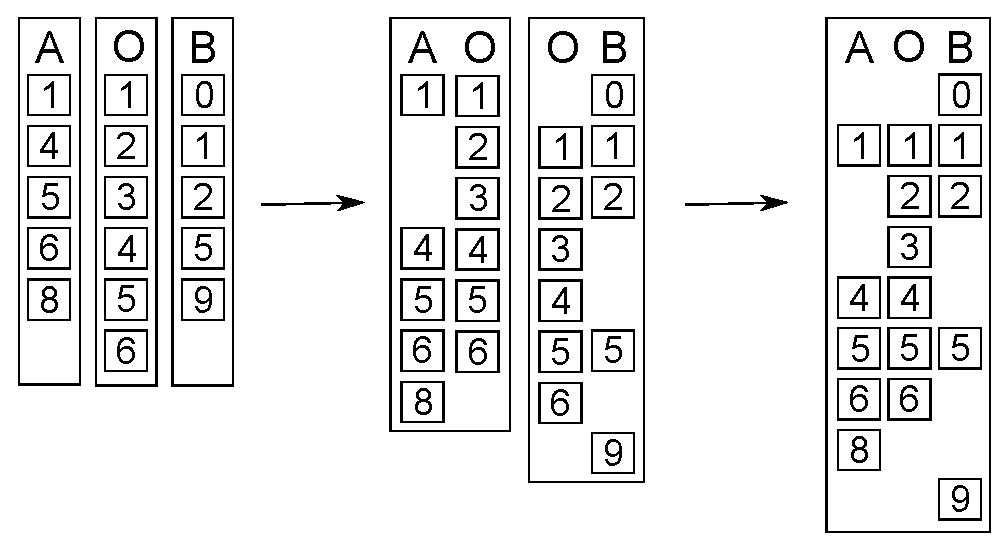
\includegraphics[scale=0.4]{drawings/eps/threewaymatching.eps}
	\caption{A run of the Three-way matching-algorithm}
\end{wrapfigure}

Given three input sequences A, O and B it will often be necessary to match these structure, and output a single sequence of matchings between the three sequences. A match is a data-structure, that contains three elements A, O and B, illustrated as a row in the result of \ref{ThreewayMatching}. An empty result in any of the three columns on each row means that there is no matching from this specific input sequence.

We will run sequence two-way matching two times on the sequence-pairs (A, O) and (O, B). Afterwards we will run a two way-matching on these two results, where equality between two two-way matches is defined as them not having an empty O-item, and having equal O-items. This will in the end giving us a list of matchings.

\begin{figure}
  \label{ThreeWayMatchingAlgorithm}
\begin{verbatim}
ThreeWayMatching(A, O, B, equality)
    AMatching <- TwoWayAllign(A, O, equality)
    BMatching <- TwoWayAllign(B, O, equality)
    return TwoWayAllign(AMatching, BMatching, (x, y) =>
                    x.O is not empty
                    y.O is not empty
                    x.O is equal to y.O
                )

\end{verbatim}
\caption{Three-way matching algorithm}
\end{figure}

\subsubsection{Reordering}
Several times in this thesis, we will have to resolve the problem where reordering of items in a sequence have happened in different branches. We will define a general three-way sequence-reordering-function, that can be given an original sequence and two reordered sequences, the result will be a single sequence where all elements are outputted in a way that can reasonably be described as a merge of the orders.

Reorderings can conflict. One example could be that the sequence \texttt{(a, b, x, c, d)} has turned into \texttt{(x, a, b, c, d)} in one branch and \texttt{(a, b, c, d, x)}. These three sequences can easily be intepreted as \texttt{x} being been moved different places in the two branches, and a conflict should be produced.

If one branch moves an item and the other branch deletes it, we will simply intepret this as a deletion. The intuition behind this, is that generally unordered sequences in programming languages will be semantically meaningless. Therefore if one user deleted it while another user simply moved it, chances are that the item is not needed anymore, and can simply be deleted.

To do a three-way reordering, the obvious entry point is to identify which items have been moved, and then apply all these moves to the output sequence. This however leads to quite a few non-trivial definitions. What is a move? It might very well be an item of the sequences, but how do we define the place that it should be moved to? Several options are available: Insert after or before a specific item, insert between items or insert at index, and many more. Each of these items, however will also present further complications, like if we choose to insert something after an item, in the output sequence, then do we do that before or after we move that item?

Further, such a move operation is not our input, and it is not clear how to calculate one from our input. Our input is three sequences with a specific order, and given those, many different move operations could be generated. The two sequences \texttt{a, b, c, d} and \texttt{a, b, d, c} can be interpreted as \texttt{c} being moved to after \texttt{d}, as \texttt{d} being placed before \texttt{c}, as \texttt{c} and \texttt{d} swapping places, and many other options. Also, figuring out the correct representation of a move in an algorithmic way can only be an uninformed guess - the users reasoning for doing a reordering might very well be grounded in context that the algorithm is unaware of.

We will look differently at reorderings. Given the input sequences we will do a matching. Such a matching will produce the actual ordering. We have earlier described small weaknesses in this approach, due to sequence alignment having more than one result, but will abstract away from that problem in this section.

A matching will contain some stable elements, and some unstable elements. The stable elements are elements where a match exists in both A, O and B. These elements, we will assume to be items that have not moved in the sequence. If something is not stable, it is either a move, an insertion or a deletion as seen in table \ref{ReorderingTable}.


\begin{figure}
\label{ReorderingTable}
\centering
\begin{tabular}{ | l | l | l || r |}
  \hline                        
   \textbf{A} & \textbf{O} & \textbf{B} & \textbf{Action by user} \\
  \hline                        
  Empty & Value & Value & "Moved from" or deleted in A \\
  Value & Value & Empty & "Moved from" or deleted in B \\
  Value & Empty & Empty & Inserted or "moved to" in A \\
  Empty & Empty & Value & Inserted or "moved to" in B \\
  Value & Value & Value & Unchanged \\
  \hline  
\end{tabular}
  \caption{How to interpret matchings in the reordering algorithm}
\end{figure}

We will iterate through each matching, and treat them as such. Distinguishing between a deletion or a "move from" is not important - we will always treat them the same: Not adding them to the output. Distinguishing between insertion and moving is quite important however. Insertions should always be inserted in the output, however moves should only be inserted to the output if they have not been deleted in the opposite branch. 

A conflicting move is a move where two "Moved to" operations exists on each list. Detecting these is a matter of looking into duplicate records in the result list. These will also be returned along with the result, and the callers of the reordering methods have the responsibility of presenting these to the user.

\begin{figure}
  \label{ThreeWayMatchingAlgorithm}
\begin{verbatim}
Reordering(A, O, B)
	matches <- ThreeWayMatcing(A, O, B, items equal)
	resultList <- [] // ResultList
	
	foreach match in matches
		if match is insertion
			add relevant item (A or B) to resultList.
		if match is move to and has not been deleted in opposite branch
			add relevant item (A or B) to resultList.
		if match is unchanged
			add item O to resultList
	conflicts = find indexes of duplicate items in resultList
	return (resultList, conflicts);
\end{verbatim}
\caption{Three-way reordering-algorithm}
\end{figure}

\subsubsection{Bi-partite graph matching}
Finding a minimum cost bipartite matching of the sets \texttt{x} and \texttt{y} can be solved in cubic time using a maximum flow algorithm as described by \citet{bipartitecost}. A prerequisite of this algorithm is however that the two sets are equal in size. Further, it assumes that the input can generate a perfect matching in the internal graph. We want to modify the bipartite graph algorithm such that it will be able to consume differently sized sets, and such it will generate the best minimum cost matching, even though it might not be a perfect matching.

The \citet{bipartitecost} algorithm starts by generating a weighted undirected graph, $G$. In this graph each item of the set is a node in the graph, and for each pair of nodes an edge is generated with the cost between them as the weight. The algorithm defines a set of prices $p$ for for each node. For $x$-nodes the initial prices are initially 0 and for $y$-nodes the initial prices is equal to the minimum weight of the incoming edges. It then creates an residual graph $G_M$ given a matching. The residual graph contains all the nodes of the original graph $G$, and further a source node $s$, and a sink node$t$. The source node has zero-cost edges to all $x$-nodes not in the matching and each $y$-node has a zero-cost edge towards the sink not in the matching. For each edge in the original graph, we will add an edge in the residual graph - if this specific edge exists in the matching we will add it as an edge from $y$ to $x$, otherwise from $x$ to $y$. The price weight of these edges will be the $price(xnode)+originalgraphweight-price(ynode)$. For each iteration of the algorithm it will update the prices such that the price in the next iteration is the current price and the cost to get from source to this node in the current residual graph.

The pseudocode for the algorithm can be found below.

\begin{figure}
\begin{lstlisting}[mathescape]
Generate $G$ from $X$ and $Y$ given a cost function
Start with $M$ to the empty set
Define $p(x)$ for $x \in X$, and  $p(y) = \underset{e \; into \; y}{\operatorname{min}} c_e$ for $y \in Y$
While $M$ is not a perfect matching
    Find a minimum-cost $s-t$ path $P$ in $G_M$ with prices $p$
    Augment along $P$ to produce a new matching $M'$
    Find a set of compatible prices with respect to $M'$
Endwhile
return M
\end{lstlisting}
\end{figure}

We want to modify this algorithm to have the following properties:

\begin{itemize}
\item It works for x and y sets of different size. 
\item It works even though a perfect matching cannot be found in the residual graph.
\item For any element not matched it should return a matching $(x, \epsilon)$ or $(\epsilon, y)$
\end{itemize}

The first challenge is relatively easy to overcome. If the sets are not equal in size, we will add nodes, auxiliary nodes, in the smallest of the two sets until the two sets are equal in size. For each auxiliary node we will add an edge to each node in the opposing set with a cost larger than the largest cost between any other pair of nodes. In the final matching, the matchings that contain auxiliary nodes should be considered as not matched; since we chose they have been matched with the highest possible weight for their edges - the rest of the matchings are definitely the minimum cost matching.
\todo{Forklar det her bedre}

The second challenge is due to the fact that the end-condition in the loop requires a perfect matching. However if any node in any of the two sets does not have a cost defined for any nodes in the opposite set, then a perfect matching is not possible. An example of such a situation could be $X={1, 2}$ and $Y={1, 3}$ with a cost function only defined for elements that are numerically equal. This is demonstrated below.

\begingroup
    \fontsize{7pt}{10pt}\selectfont
\begin{tabular}{ p{5.5cm} | p{5.5cm} }
	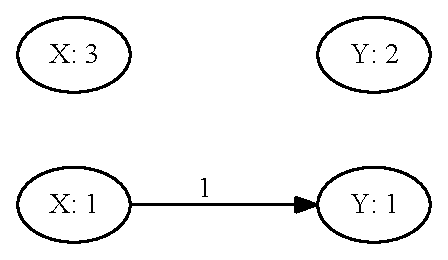
\includegraphics[scale=0.3]{drawings/eps/TwoWayCostMatchingNotPerfect/1it0.eps} &
    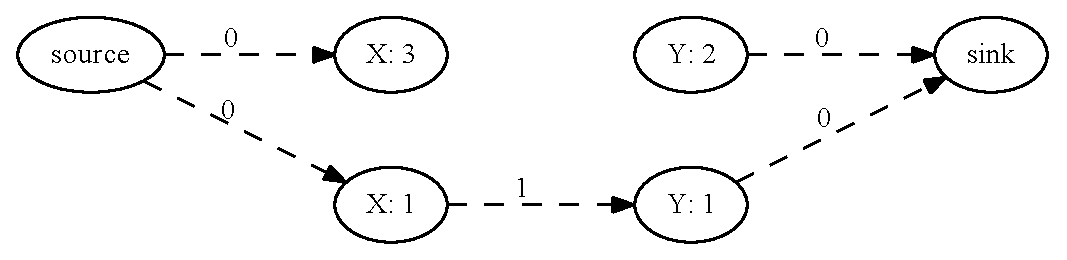
\includegraphics[scale=0.3]{drawings/eps/TwoWayCostMatchingNotPerfect/1it1.eps} \\
	Initial graph for the sets and cost function. &
    The first residual graph. \\ \\ \hline \\

    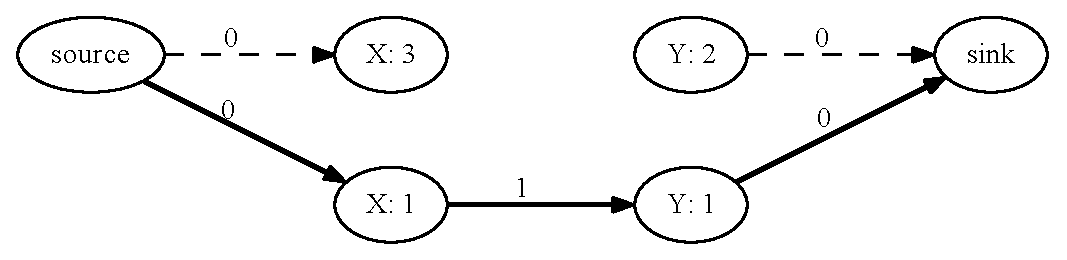
\includegraphics[scale=0.3]{drawings/eps/TwoWayCostMatchingNotPerfect/1it2.eps} &
    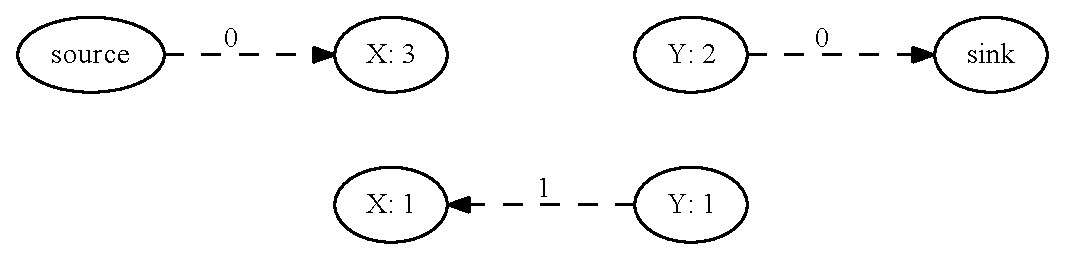
\includegraphics[scale=0.3]{drawings/eps/TwoWayCostMatchingNotPerfect/1it3.eps} \\
	Running dijkstra finds a matching. &
	In the second residual graph, all possible matchings have been found, but the matching is still not a perfect matching. \\ 
\end{tabular}

\endgroup

When our algorithm reaches the second iteration, the matching is still not perfect for the entire graph. The problem is that one or more edges have no edges in the initial graph, and as such the solution seems simple: Remove and remember nodes with no costs generated for them. One argument against this being the solution, would be the situation where the X-node 1 actually has a cost for the Y-node two. In the original algorithm, the matching would still not perfect on the graph. However this problem will be solved by auxiliary nodes being inserted on the graph generation.

The algorithm now becomes:

\begin{figure}
\begin{lstlisting}[mathescape]
Generate $G$ from $X$ and $Y$ given a cost function.
	- Inserting auxiliary nodes if the $|X| \neq |Y|$
	- Store items of $X$ and $Y$ that has no cost.
	    Do not add them to $G$.
	    
Start with $M$ to the empty set.
Define $p(x)$ for $x \in X$, and  $p(y) = \underset{e \; into \; y}{\operatorname{min}} c_e$ for $y \in Y$
While $M$ is not a perfect matching
    Find a minimum-cost $s-t$ path $P$ in $G_M$ with prices $p$
    Augment along $P$ to produce a new matching $M'$
    Find a set of compatible prices with respect to $M'$
Endwhile

Return the union of these three sets:
    For matchings with an auxiliary node, select $(x, \epsilon)$ or $(\epsilon, y)$
    For other matchings select the matching.
    For each item not added to $G$, select $(x, \epsilon)$ or $(\epsilon, y)$

\end{lstlisting}
\end{figure}



\subsubsection{Three-way cost matching}
Matching the members $(l_1, l_2, ..., l_{size(l)})$, $(b_1, b_2, ..., b_{size(b)})$ and $(r_1, r_2, ..., r_{size(r)})$ will be done by making a bipartite matching between the pairs $(b, l)$ and $(b, r)$, and afterwards matching the matching on the base items.

Given the left to base and right to base matching, we will do another unordered matching on the base-items.

\todo[inline]{We could probably just sort them after $b$-items, and then do an ordered matching.}

An over approximation of the running time here will be  $3*max(x, y, z)^3$.

\subsubsection{TODO}

- Unordered matching of different sized bipartite matching
- Chunking of three-way matches
- Prioritymatching
- Diff3.Merge

\subsection{Merging classes}
Classes, namespaces etc are structures.

file merge(base, left, right)
    if(nodes are unordered)
        unorderedmatch(base, left, right)
    else if(nodes are ordered)
        orderedmatch(base, left, right);

file unorderedmerge(base, left, right)
    var bl = match B and Ls children given cost-function
    var br = match B and Rs children given cost-function
    var zip = match bl and br on same base object.

    var members = [];

    foreach(match in zip)
        if(match exists in all)
            member.add(m, merge(base, left, right));
        if(match was inserted in B)
            member.add(m, m.B);
        if(match was inserted in A)
            member.add(m, m.A);
    
    members = mergeorder(l, b, r, members);

    return recreate(b, l, r, members);
    

file orderedmerge(base, left, right)
    run diff3 algorithm on the source text of base, left, right
    if a conflict happens, do a three-way matching-tree matching on the trees. instead.
    use this three-way match to reconstruct a new tree.



\subsubsection{Function similarity measure}
Doing cost-based matching, means we also will have to define function similarity measures. This function will have to be run for each $(l, b)$ and $(r, b)$-pair, which means it is important to keep the running time low.

Four overall parameters are obvious as similarity measures:

\begin{enumerate}
    \item The identifier of a class member.
    \item The parameters of a class member.
    \item The modifiers of a class member.
    \item The body of a class member.
\end{enumerate}

For identifiers equal strings will of course have to be the lowest cost. Besides that, one could think up different string similarity measures that would allow different renames of a member to have lower costs than others.
\todo[inline]{Needs to elaborate alot}

\subsubsection{Ordering of outputted class members}
The end result of the matching algorithm will be a set of merged class members. 

Conflicts might exists if two users have moved the same function into different places in the left and right branches, but that is the only case where user intervention should be needed. However there are quite a few cases of reordering operations, where the answer of where to actual position a function in the output is simply undefined. 

For example:

A = { a, b, d, c }
O = { a, b, c, d }
B = { a, c, d, b }


Reordering items 

First we do a three-way sequence matching of base, left and right. 

A deletion is a matching from an item in base to null.
An insertion is a matching from null to an item in left.
In a matching, a move will simply be represented as an insertion and a deletion.



Observations:
- If a node is deleted in either left or right, it should be deleted even if it has been reordered. (However conflict if the content has been modified)
- If a deletion happens 


\todo{Match default? Forrest or tree? Do we allways know that the root node matches?}



\subsubsection{Merging functions}
Foreach function, write about:

Intended input.
Purpose of the function.
Conflict behaviour
Tricks that are not obvious.
Intended output.

\paragraph{Merging nodes}
\texttt{MergeNode} handles merging of single nodes. It will take three input values; A, O and B, and return a syntactically valid string, which is the merge of those three input values. It handles the input as a matching and will conclude insertion or deletion if appropriate. Further it assumes that all input nodes are of the same type.

\begin{itemize}
	\item If O is null and either A or B is null it treats the input as an insertion, and returns the inserted value.
	\item If O is not null, and A or B is null it treats the input as a deletion. It will verify that no changes has happened in the other branch and return either a conflict, or empty.
\end{itemize}

Otherwise it will treat the input as a merge of the two branches A and B. From a concrete syntax perspective, we will have to look into two factors of the current node, to see what to return:

\begin{itemize}
	\item The concrete syntax that this node emits.
	\item The concrete syntax that each child of this node emits.
\end{itemize}

The responsibility of MergeNode is to only return the the exact syntax needed for these specific node. Any work of generating concrete syntax for children will be handled by a recursive call to MergeNode. For example a method invocation will simply generate the opening and closing parenthesis, while the argument list will simply be passed to another invocation, as well as the method-expression. This breakdown makes the merging of most nodes quite trivial.

Some nodes only consists of tokens: A function name, a string literal, an integer, a keyword and so forth. For these kind of nodes, we will simply check if only one of the branch nodes differs, and if this is the case, return that, and otherwise return a conflict, as can be seen in \ref{MergeToken}


\begin{figure}
  \caption{The main entry point for the Syntax Tree merging}
  \label{MergeNode}
\begin{verbatim}
MergeNode (of method declerations and below)
    if A or B has been deleted.
        if(others havent changed)
            return nothing;
        else
            return conflict;
            
    if A or B has been inserted
        return A or B
        
    if(nodes is fixed structural node)
        retur merge of each child and own structure
    if(node is a content-node) 
        return the token merge
    if(nodes is a list) (parameterlist, argumentlist)
        return listmerge of cost function
    if(node is a block)
        Merge conditions if they exist.
        Merge Substatemnetlists.
        return the two merges.
        

\end{verbatim}
\caption{A fixed structural node is nodes that has a fixed number of children, that are easily merged - like methods declerations, expressionsstatements, invocations, memberaccesses, single arguments. A content node is a node which is generated from a single token.}
\end{figure}


\begin{figure}
  \caption{Merging tokens}
  \label{MergeToken}
\begin{verbatim}
MergeToken(A, O, B)
    if all equal
        return value
    if one has changed
        return changed value
    if both has changed 
        if A != B
            return conflict
        return A
\end{verbatim}
\end{figure}

\paragraph{Merging lists}
There are primarily two types of list that we want to merge: ParameterLists and ArgumentLists. Parameterlists are the pair of types and identifiers found in method declarations, where argument-lists are expressions found in invocations of methods. Modification of these can be for several reasons.

\begin{itemize}
	\item Modifications of parameter-lists can be reorderings with no semantic meaning. Further it can be additions or removals of a parameter. These will often also be accompanied by some change in the behaviour of a method.
	\item Modifications of argument-lists can be done as a consequence of change in a parameter list other places in the syntax-tree. They can also be done simply because another expression or value needs to be passed into a function, or because the user intends to call another overload of the method.
\end{itemize}

We will do an unordered matching of the lists, and then do a reordering, and filtering of the output. The returned list is a list that tries to preserve any reordering, and that has filtered items in the sequence that did not exist in either of the two branches. This will hopefully ensure that:

\begin{itemize}
	\item Since the reordering uses the exact same algorithm a merge of parameter- and argument-lists will produce compatible output, provided that the cost function matches in the same way on both branches.
	\item All items that existed in the branches will exist in the output of this function. 
	\item Conflicts can be marked easily for the user.
\end{itemize}

The cost between a pair of parameters can be boiled down the question of how similar the type of the parameter is, and how similar the name is. Similarity of type can be measured as closeness in the class hierarchy. String similarity can be measured in quite a few ways. In our case we will want to keep the runtime low and as such we will keep to a simple and exact scheme of similarity of both.

The cost of the argument-lists is much harder to define. An argument is an expression, so the obvious thought would be to look into what type that expression will have. This information, however, is not very often available when looking at a single class. The idea here must be to try to find to find similar matches, and link only the expressions that are most similar. We will therefore use the similarity function as cost function for these. 

\todo{example}

\begin{figure}
  \caption{Merging tokens}
  \label{MergeToken}
\begin{verbatim}
Listmerger (A, O, B, cost)
    match A, O, B after cost.
    (merge, conflicts) = FilterReorderMergeContent(a, o, b, match)
    foreach conflict
        add the warning to the two conflicts

\end{verbatim}
\end{figure}

\paragraph{Merging blocks}
erging blocks and 


What are the right properties of a merge?

\begin{figure}
  \caption{Merging statement lists}
  \label{MergeStatementList}
\begin{verbatim}
MergeStatementList (A, O, B)
    try  a textual merge of the statements.
    If that does not work:
        Do a prioritydiff of the statements
        for all chunks
            if chunk is primaryequal
                return one of the sides
            else if chunk is secondary equal
                chunkmerge!
            else if one chunk is empty (deletion or insertion)
                chunkmerge!
            else 
                attempt uneven merging

\end{verbatim}
\end{figure}

\begin{figure}
  \caption{Merging uneven branches}
  \label{MergeToken}
\begin{verbatim}
MergeUneven (A, O, B)
    Flatten the three list. Any statement with a subblock, has the statements in this subblock added to it, keeping parent item mapping
    Prioritydiff the three flattened lists.

    Parentitems = [nil, nil, nil]

    foreach chunk
        if stable chunk
            if(lastitem O is null and B and A is not)
                return conflict

            if(any parentitem has changed since last iteration)
                if(if last parent item as a block block)
                    print "}"
                if(if a current parent item exists)
                    print(merge(parentitems))
                    if(currentparentitems merrits block)
            
            print merge(child item)

        else 
            if A or B is insertion
                add A or B, updating their correspinding parentitem,
                and adding starting and ending items, as above
\end{verbatim}
\end{figure}


-- Equality
-- Similiarity
-- Matching blocks and lists
-- Merging.
--- Merging inserted blocks.

\clearpage
\section{Evaluation}

\clearpage
\section{Conclusion}

\clearpage

\bibliographystyle{plainnat}
\bibliography{libary}

\end{document}

